\chapter{Resultados}

\graphicspath{ {/var/www/html/meninadasbalas/projetc/monografia/latex/images/} }

% @@@@@@@@@@@@@@@@@@@@@@@@@@@@@@@@@@@@@@@@@@@@@@@@@@@@@@@@@@@@@@@@@@@@@@@@@@@ %
% @@@@@@@@@@@@@@@@@@@@@@@@@@@@@@@@@@@@@@@@@@@@@@@@@@@@@@@@@@@@@@@@@@@@@@@@@@@ %
\section{Desenvolvimento}
Para atingir os objetivos colocados e requerimentos do cliente, além de todo o processo de construção e configuração do site, tivemos que construir 2 módulos, adaptar versão de 1 e criar 1 sub-tema a partir de uma tema base.

% =========================================================================== %
\subsection{Módulo 1 - MBC Master}
O primeiro módulo foi chamado de MBC Master. Sua função é criar plugins de formatação de campos para o site. O campo de imagem de um produto pode ter carregadas até 10 imagens, porém em alguns casos como na lista de produtos da página inicial, apenas um imagem pode ser exibida. Para executar esta tarefa, foi copiado a classe de formatação do núcleo do Drupal para este módulo e modificada, para trazer apenas a primeira imagem. Por esta razão o plugin foi chamado de FirstImageFormatter.

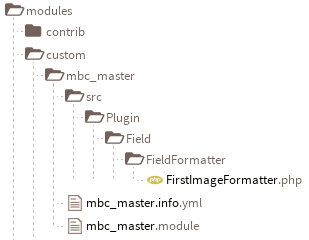
\includegraphics{mbc_master}

% =========================================================================== %
\subsection{Módulo 2 - MBC Review}
Este módulo foi criado com o objetivo de prover um método para o administrador do site enviar e-mail para usuários pedindo Reviews de produtos ou Opiniôes sobre a empresa, prover um link exclusivo para criação destes conteúdos que vai neste e-mail, que reconhece automaticamente o usuário e não publique este conteúdo, deixando-o para moderação do administrador.

% =========================================================================== %
\subsection{Módulo Adaptado - TinyPNG}
Por ser um módulo bem simples que utiliza uma biblioteca externa para fazer a minificação, a adptação deste módulo foi bem simples. Uma função que é executada quando uma entidade (conteúdo) é salva foi utilizada e usada a biblioteca tinify \url{packagist.org/packages/tinify/tinify} para executar a minificação das imagens. Além disso, o módulo adiciona uma página administrativa para ser gerenciada a chave da API do serviço, que pode ser obtida no site \url{https://tinypng.com/}.

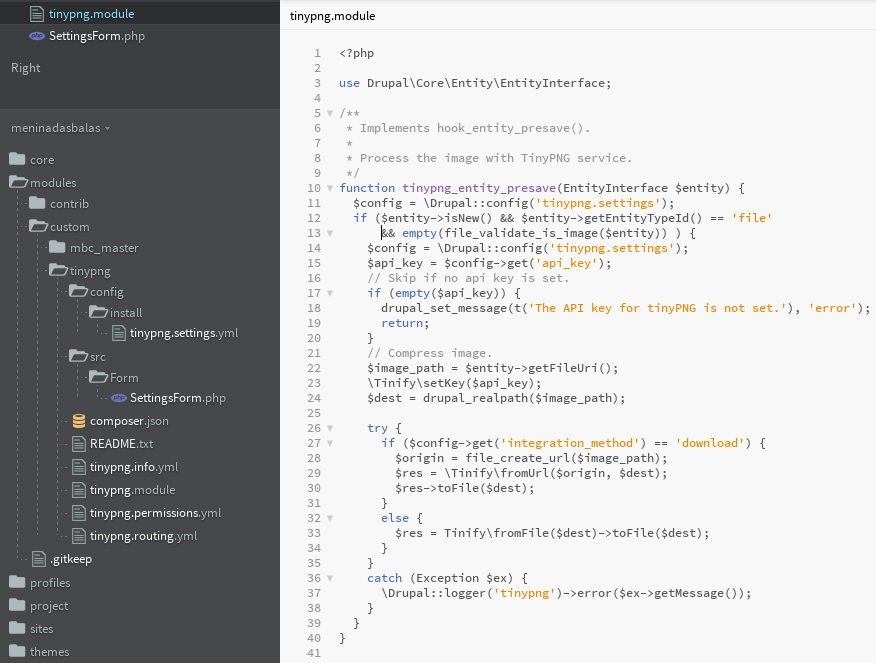
\includegraphics{tinypng2}

% =========================================================================== %
\subsection{Sub-tema - MBC Theme}
Todo front-end do site é construido neste sub-tema. A base é o framework Bootstrap e seu tema para Drupal 8. 

\subsubsection{Gulp}
O automatizador de tarefas Gulp foi utilizado para algumas das principais tarefas de desenvolvimento deste tema como descrito anteriormente e o resultado foi um fluxo de front-end bem mais rápido, sólido e seguro. Todas as ferramentas funcionaram como previsto e todo o código de LESS e Javascript que foram necessários, seguem um padrão de código bem definido e não possuem estruturas inseguras.

\subsubsection{LESS}
Para os arquivos Less, que vão gerar o CSS do site, utilizamos uma estrutura modular, onde cada bloco e página do site tem seu próprio LESS, resultando em arquivos com menos 100 linhas, de facil manutenção e preparados para melhorias no carregamento do CSS pelas páginas do site.

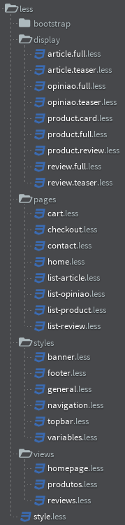
\includegraphics{less}

\subsubsection{Templates Twig}
O Drupal 8 tem um sistema de templates que são utilizados para montar as páginas. Para customizar estes templates, temos que sobrescreve-los. Nosso tema base já possui vários templates sobre-escritos do núcleo e nós nos baseamos nestes para fazer os nossos. Até o momento foram necessários mais de 20 templates e com as melhorias sendo feitas constantemente no site, mais serão criados.

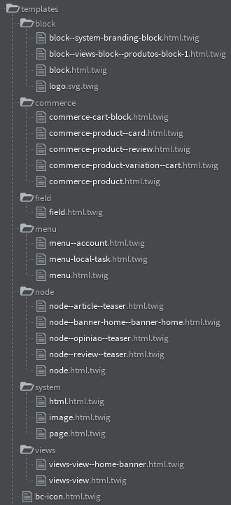
\includegraphics{templates}

% @@@@@@@@@@@@@@@@@@@@@@@@@@@@@@@@@@@@@@@@@@@@@@@@@@@@@@@@@@@@@@@@@@@@@@@@@@@ %
% @@@@@@@@@@@@@@@@@@@@@@@@@@@@@@@@@@@@@@@@@@@@@@@@@@@@@@@@@@@@@@@@@@@@@@@@@@@ %
\section{Performance}

Medimos a performance do site pelo serviço préviamente apresentado chamado GTMetrix. As notas obtidas são bem constantes a cada análise, porém o tempo de resposta do servidor pode mudar significativamente. Utilizamos então uma média de 10 análises para apresentar este resultado.


